\chapter{ASAI - Adaptive Statistical Analysis for Images}
\label{Appendix A}


\section{Motivation for Development}

Surface roughness analysis, a staple technique in nano-tribology and the Krim nano-tribology group, though not particularly difficult for an individual image, quickly becomes time consuming and tedious as the number of images grows. Typically, using third-party software to assess the images, then using OriginPro (TM?) to plot and interpret those quantities, analysis of a single image would require a minimum of 10 minutes. Use of the ASAI package, written on the foundation of Krim Group roughness/fractal surface analysis principles, reduced the time cost for analysis of a single image to, on average, 10 seconds. In the event that there is a need to combine the roughness analysis output from multiple AFM images or to quickly change graph titles, time-savings are again added to the value of the ASAI system.

\section{Principles of Operation}


This code was developed around methods well-established in Dr. Krim's previous work including [refs for Krim surface roughness characterization]

Adaptive Analysis by Adj-R2 maximization

\section{Future Development Paths}

Generalizable to any matrix, square or otherwise....

\begin{figure}[hbtp]
	\centering
	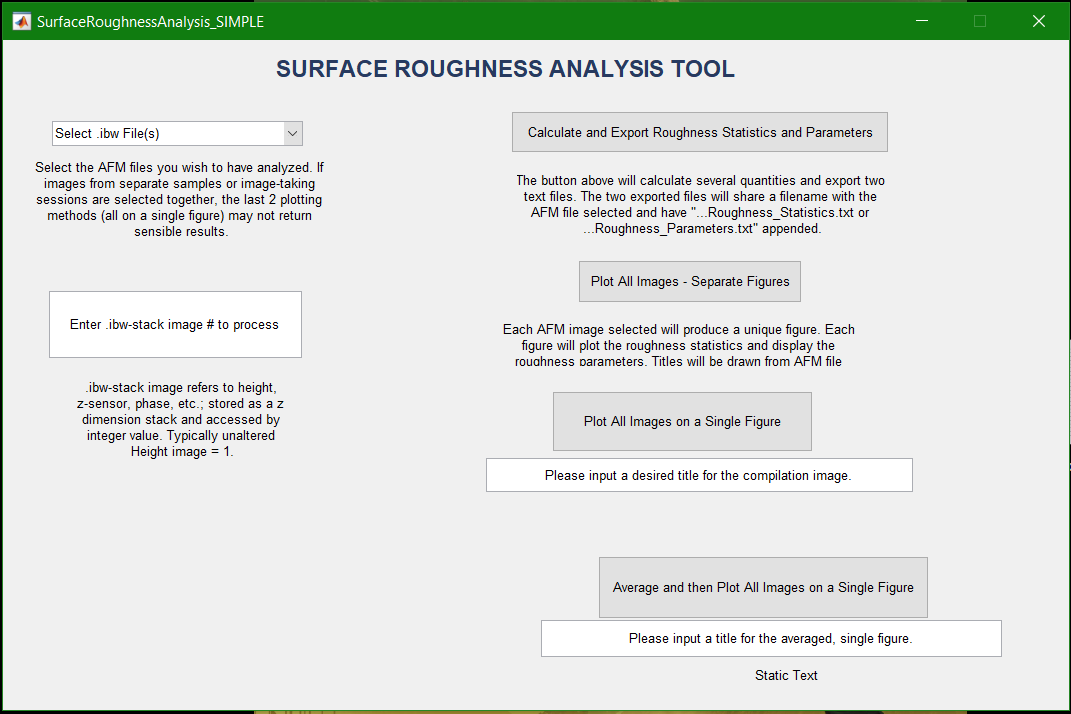
\includegraphics[width=1.0\textwidth]{Appendix-A/ASAI_GUI}
	\caption{ASAI, a MATLAB-based image analysis package, utilizes a simple graphical user interface (GUI) to provide a simple experience for users, regardless of programming skill.}
	\label{figA1: ASAI_GUI}
\end{figure} 


\section{ASAI Manual !!! Incomplete}

%%%%%%%%%%%%%%%%%%%%%%%%%%%%%%%%%%%%%%%%%%%%%%%%%%%%%%%%%
%%%%%%%%%%%%%%%%%%%%%%%%%%%%%%%%%%%%%%%%%%%%%%%%%%%%%%%%%

Adaptive Statistical Analysis for Images (ASAI) README

%%%%%%%%%%%%%%%%%%%%%%%%%%%%%%%%%%%%%%%%%%%%%%%%%%%%%%%%%
%%%%%%%%%%%%%%%%%%%%%%%%%%%%%%%%%%%%%%%%%%%%%%%%%%%%%%%%%

(c) 2017 North Carolina State University, Colin K Curtis, Jacqueline Krim

Author (code) =	Colin K Curtis
contact = 	colinkcurtis@gmail.com
github.com/colinkcurtis

Methods = Jacqueline Krim, citations: 
Panella, Krim. 1994.  "Adsorbate surface tension effects for isotherms
recorded on fractally rough surfaces"

Berman, Krim. 2012. "Impact of oxygen and argon plasma exposure on the
roughness of gold film surfaces"


%%%%%%%%%%%%%%%%%%%%%%%%%%%%%%%%%%%%%%%%%%%%%%%%%%%%%%%%%
%%%%%%%%%%%%%%%%%%%%%%%%%%%%%%%%%%%%%%%%%%%%%%%%%%%%%%%%%

Setup
%%%%%

There are several critical files which this package requires:

-SurfaceRoughnessAnalysis\_SIMPLE.fig  	(GUI component)
-SurfaceRoughnessAnalysis\_Simple.m    	(primary code)
-IBWread.m				(code for reading-in IBW files, a typical AFM output file type)				
-readIBWbinheader.m			(support code for IBWread.m)
-readIBWheaders.m			(support code for IBWread.m)

Ensure that all 5 objects, listed above, are placed into a single
directory. In the MATLAB IDE, 'Add' this directory/folder 'to the path'
so that MATLAB has all of the functional pieces within its scope.

If the IBW/image files which you wish to process are not located
in the directory along side the 5 aforementioned pieces of code,
"Add to path" the directory where your IBW/image files are stored.
If you do not add this directory to the MATLAB path, running the
program on a file outside the path will result in MATLAB errors.




%%%%%%%%%%%%%%%%%%%%%%%%%%%%%%%%%%%%%%%%%%%%%%%%%%%%%%%%%
%%%%%%%%%%%%%%%%%%%%%%%%%%%%%%%%%%%%%%%%%%%%%%%%%%%%%%%%%



%%%%%%%%%%%%%%%%%%%%%%%%%%%%%%%%%%%%%%%%%%%%%%%%%%%%%%%%%
%%%%%%%%%%%%%%%%%%%%%%%%%%%%%%%%%%%%%%%%%%%%%%%%%%%%%%%%%
%%%%%%%%%%%%%%%%%%%%%%%%%%%%%%%%%%%%%%%%%%%%%%%%%%%%%%%%%
%%%%%%%%%%%%%%%%%%%%%%%%%%%%%%%%%%%%%%%%%%%%%%%%%%%%%%%%%


\section{ASAI Code - Complete}

\begin{sloppypar}
\begin{lstlisting}

%
%%% --- GUI builder, from the MATLAB editor
%

function varargout = SurfaceRoughnessAnalysis_SIMPLE(varargin)
% SURFACEROUGHNESSANALYSIS_SIMPLE MATLAB code for
% SurfaceRoughnessAnalysis_SIMPLE.fig
%      SURFACEROUGHNESSANALYSIS_SIMPLE, by itself, creates a new
%      SURFACEROUGHNESSANALYSIS_SIMPLE or raises the existing singleton*.
%
%      H = SURFACEROUGHNESSANALYSIS_SIMPLE returns the handle to a new
%      SURFACEROUGHNESSANALYSIS_SIMPLE or the handle to the existing
%      singleton*.
%
%      SURFACEROUGHNESSANALYSIS_SIMPLE('CALLBACK',hObject,eventData,handles
%      calls the local function named CALLBACK in
%      SURFACEROUGHNESSANALYSIS_SIMPLE.M with the given input arguments.
%
%      SURFACEROUGHNESSANALYSIS_SIMPLE('Property','Value',...) creates a
%      new SURFACEROUGHNESSANALYSIS_SIMPLE or raises the existing
%      singleton*.  Starting from the left, property value pairs are
%      applied to the GUI before SurfaceRoughnessAnalysis_SIMPLE_OpeningFcn
%      gets called.  An unrecognized property name or invalid value makes
%      property application stop.  All inputs are passed to
%      SurfaceRoughnessAnalysis_SIMPLE_OpeningFcn via varargin.
%
%      *See GUI Options on GUIDE's Tools menu.  Choose "GUI allows only one
%      instance to run (singleton)".
%
% See also: GUIDE, GUIDATA, GUIHANDLES

% Edit the above text to modify the response to help
% SurfaceRoughnessAnalysis_SIMPLE

% Last Modified by GUIDE v2.5 28-Nov-2016 16:13:05

% Begin initialization code - DO NOT EDIT
gui_Singleton = 1;
gui_State = struct(		'gui_Name',       mfilename, ...
'gui_Singleton',  gui_Singleton, ...
'gui_OpeningFcn', @SurfaceRoughnessAnalysis_SIMPLE_OpeningFcn, ...
'gui_OutputFcn',  @SurfaceRoughnessAnalysis_SIMPLE_OutputFcn, ...
'gui_LayoutFcn',  [] , ...
'gui_Callback',   []);
if nargin && ischar(varargin{1})
gui_State.gui_Callback = str2func(varargin{1});
end

if nargout
[varargout{1:nargout}] = gui_mainfcn(gui_State, varargin{:});
else
gui_mainfcn(gui_State, varargin{:});
end
% End initialization code - DO NOT EDIT

% --- Executes just before SurfaceRoughnessAnalysis_SIMPLE is made visible.
function SurfaceRoughnessAnalysis_SIMPLE_OpeningFcn(hObject, eventdata,...
handles, varargin)
% This function has no output args, see OutputFcn. hObject    handle to
% figure eventdata  reserved - to be defined in a future version of MATLAB
% handles    structure with handles and user data (see GUIDATA) varargin
% command line arguments to SurfaceRoughnessAnalysis_SIMPLE (see VARARGIN)

% Choose default command line output for SurfaceRoughnessAnalysis_SIMPLE
handles.output = hObject;

% Update handles structure
guidata(hObject, handles);

% UIWAIT makes SurfaceRoughnessAnalysis_SIMPLE wait for user response (see
% UIRESUME) uiwait(handles.figure1);

% --- Outputs from this function are returned to the command line.
function varargout = SurfaceRoughnessAnalysis_SIMPLE_OutputFcn(hObject, ...
eventdata, handles) 
% varargout  cell array for returning output args (see VARARGOUT); hObject
% handle to figure eventdata  reserved - to be defined in a future version
% of MATLAB handles    structure with handles and user data (see GUIDATA)

% Get default command line output from handles structure
varargout{1} = handles.output;

% --- Executes on selection change in popupmenu1.
function popupmenu1_Callback(hObject, eventdata, handles)

global A
global AFMMetaData
global FileName
global IBWFiles
global Space

Space = ' '; %Just a space used in glueing together strings throughout 
...the program!

% The lines below take important information from the AFM file, such as
% file name, Scan Size (physical and # pixels), and Imaging mode, and save
% them for calculation or later use on the graphs to be plotted
[FileName, PathName, filterindex] = uigetfile('*.ibw',... 
'Select the ibw file', 'MultiSelect','on');
if ischar( FileName ), FileName = { FileName };  % for uigetfile,
end										% single file read-in is trouble

A = length(FileName);        % A variable we use in for loops to follow
IBWFiles = cell(1,A);       % This will hold the image data itself!!!

for i= 1:A                % Look through all of the files selected above

Q = FileName{i};        % Assign the filename to variable Q  
P = IBWread(Q);         % This fcn reads in and assigns ibw files to P
IBWFiles{i} = P;        % Creates a cell array of all the read-in files
tempWaveNotes = P.WaveNotes;  % this

AFMMetaData{i} = textscan(tempWaveNotes, '%s','delimiter', '\n');

%     assignin('base','IBWFiles',IBWFiles);       % Adds the cell array
%     just created to the workspace assignin('base','FileName',FileName);
end

%    assignin('base','AFMMetaData',AFMMetaData);

if isequal(FileName,0) % in case no file is selected, a msg is displayed
disp('User did not select files')

else                    % the filenames of the files read in are displayed
disp(['user selected the .ibw file(s):', fullfile(PathName, FileName)])
end


% --- Executes during object creation, after setting all properties.
function popupmenu1_CreateFcn(hObject, eventdata, handles)

if ispc && isequal(get(hObject,'BackgroundColor'), ... 
get(0,'defaultUicontrolBackgroundColor'))
set(hObject,'BackgroundColor','white');
end


function edit2_Callback(hObject, eventdata, handles)

get(hObject,'String');


% --- Executes during object creation, after setting all properties.
function edit2_CreateFcn(hObject, eventdata, handles)

if ispc && isequal(get(hObject,'BackgroundColor'), ... 
get(0,'defaultUicontrolBackgroundColor'))
set(hObject,'BackgroundColor','white');
end


function edit3_Callback(hObject, eventdata, handles)

get(hObject,'String');


% --- Executes during object creation, after setting all properties.
function edit3_CreateFcn(hObject, eventdata, handles)

if ispc && isequal(get(hObject,'BackgroundColor'), ...
get(0,'defaultUicontrolBackgroundColor'))
set(hObject,'BackgroundColor','white');
end



function edit5_Callback(hObject, eventdata, handles)

get(hObject,'String');

% --- Executes during object creation, after setting all properties.
function edit5_CreateFcn(hObject, eventdata, handles)

if ispc && isequal(get(hObject,'BackgroundColor'), ...
get(0,'defaultUicontrolBackgroundColor'))
set(hObject,'BackgroundColor','white');
end

%
%%% ROUGHNESS STATISTICS AND ROUGHNESS PARAMETER CALCULATION AND FILE
%%% EXPORT
%
function pushbutton1_Callback(hObject, eventdata, handles)

format longeng    % makes it so we can see numbers which are different ...
% by orders of magnitude

global A
global AllImageStats
global AFMMetaData
global AllExpFitCoefficients
global AllLinFitCoefficients
global AllRoughnessParameters
global DataForFitting
global FileName
global FirstExpFit
global FirstExpFitOptions
global IBWFiles
global LastLinearPoint
global LinFit
global PhysicalScanSize
global Pixels
global SquareRootofLastWeight
global y0Start

AllImageStats = cell(1,A);     % pre-allocates a cell array which will 
% store the calculated length/RMS matrices
DataFileHeader = cell(1,3); %This will be the header for the 
%"____statistics.txt" export text file
DataFileHeader = {'Length(A)','RMS Roughness(A)','STD of Roughness(A)'};
ImageSelect = get(handles.edit2, 'string');
ImageSelect = str2double(ImageSelect);
Pixels = zeros(1,A);
VarianceOfLogRMSValues = 1;

disp '***Roughness Analysis Has Begun***'

for i = [1:A]                       
tempCELL = IBWFiles{i};       % picks out a single image file-set 
% from the cell array

PickHeight = tempCELL.y; % picks out all of the height data 
% (for all of the available types, 
%phase, amplitude, height, etc) from the file

PickImage = PickHeight(:,:,ImageSelect);  % selects the 6th image, 
%in my case the modified height, THIS NEEDS TO BE USER-INPUT

Pixels(1,i) = length(PickImage);     % # of pixels for a square image 
% in EACH DIMENSION

N = log(Pixels(1,i))/log(2);         % This will control the outer-most
% for loop for each image, below

tempStringforPhysicalScanSize= AFMMetaData{i}{1}{1};  
% This will go into the AFM-file meta-data to find physical image size

clippedString = strrep(tempStringforPhysicalScanSize,'ScanSize: ','');

PhysicalScanSize = 10e9*str2double(clippedString); 
% Gives the square-dimension of the image in Angstroms

AngstromLength = zeros(N,1);    
% pre-allocate a matrix to hold length values in Angstroms

RMSValues = zeros(N,1);         
% pre-allocate a matrix to hold RMS Roughness values for each length-scale

LogAngstromLength = zeros(N,1);

LogRMSValues = zeros(N,1);

LogRMSWeights = zeros(N,1);

LogSTD = zeros(N,1);

STD = zeros(N,1);               
% pre-allocate a matrix to hold the uncertainty for each RMS Roughness value

for j = [1:N]                 
% this outer loop will reset for each image selected

PixelsPerSquare = 2^j;      
% determines the number of pixels (for each dimension) to examine

NumberOfValuesToAVG = (Pixels(1,i)/PixelsPerSquare)^2;    
% With each new length scale, the number of values changes as x^2

RMSHolder = zeros(NumberOfValuesToAVG,1);       
% pre-allocates a matrix in which the STD from each small square

m = 1; % is saved until they can be averaged and STD calculated                                                 

ADD = 2^j-1;        
% ADD is an incrementer which adjusts to the size of the box being
%  used for STD calculations, below

for k = [1:PixelsPerSquare:(Pixels(1,i)-PixelsPerSquare+1)]          
%in the x-direction, this loop takes us across the pixels
%by bits = to the square size defined prev as "pixel per square"
incrementk = k + ADD;                                                     

for l = [1:PixelsPerSquare:(Pixels(1,i)-PixelsPerSquare+1)]          
% runs through the y values    
incrementl = l + ADD;                
RMSHolder(m) = std2(PickImage(k:incrementk,l:incrementl));    
% The heart of things: finds the std for each small square
m = m + 1;
%increments the list of STDs forward to save the next value
end
end

StdOfRMS = std(RMSHolder)*1e10;         
% Finds the STD/uncertainty for all the little-square calculations
RMSMean = mean(RMSHolder)*1e10;         
% averages the measurements from each small square
STD(j) = StdOfRMS;                      
% Stores the avg STD value in a vector for calculation of LogSTD 
% in the next line
LogSTD(j) = STD(j)/(RMSMean*log(10));   
% This is the fractional uncertainty of LogRMSValues, below   
RMSValues(j) = RMSMean;                 
%Adds to the average from above to a list which saves 
% the values across length scales, for each image
LogRMSValues(j) = log10(RMSMean);       
% this will be the y-value we use for "roughness statistics" and 
%calculating roughness parameters

tempAngstromLength =PhysicalScanSize*(PixelsPerSquare/Pixels(1,i));  
% need to turn pixel values into real length values!
AngstromLength(j) = tempAngstromLength;                               
% creates a list of the real lengths we have just calculated
LogAngstromLength(j) = log10(tempAngstromLength);                     
% we want log-log for roughness parameter calculations, 
% this is the x-values vector

if j ~= N
VarianceOfLogRMSValues = LogSTD(j)*LogSTD(j);  
% We calculate the weights for each point for the final fit
LogRMSWeights(j) = 1 / VarianceOfLogRMSValues; 
% The weight, for each data point, is  1 / variance
else
tempFit = fitlm(LogAngstromLength,LogSTD);   
% so... above we could find the weights for fitting quite easily

tempSlope = tempFit.Coefficients{2,1};       
% but the last RMS roughness measurement, of the ENTIRE AFM image

tempy0 = tempFit.Coefficients{1,1};          
% produces only ONE value. Thus, there is no obvious 
% STD/uncertainty to use!

SquareRootofLastWeight = tempSlope(1,1)*LogAngstromLength(j)+tempy0(1,1); 

LogSTD(j) = SquareRootofLastWeight;          
% So, here we fit the uncertainties of all of the 
% smaller RMS roughness values

LastWeight = SquareRootofLastWeight^2;       
% which were calculated, used to extrapolate what might expect

LogRMSWeights(j) = 1 / LastWeight;           
% The uncertainty of the last single RMS roughness measurements
% to be
end

XandYandZ = [AngstromLength RMSValues STD LogAngstromLength ...
LogRMSValues LogSTD LogRMSWeights]; 
% creates a 6-column matrix with important values
y0Start = LogRMSValues(end);         
% this is  used to give the exponential fit a place to begin 
% its search for a y-intercept

end

OutputTemp1 = FileName{i};
OutputTemp1 = OutputTemp1(1:end-4);
NameForTextFile = sprintf('%s_Roughness_Statistics.txt',OutputTemp1);
AllImageStats{1,i} = {NameForTextFile; DataFileHeader; XandYandZ};              
% Adds the 3-column list to a cell array to store for all selected
% images

%assignin('base','AllImageStats',AllImageStats); % DIAGNOSTIC: Saves
%the above stat lists for all of the images to the workspace
% useful as a diagnostic tool
end

LS = 'Length Scale [Angstroms]', RR = 'RMS Roughness [Angstroms]', ...
STDRR = 'STD of RMS Roughness [Angstroms]';
LOGLS = 'log(Length Scale)', LOGRR = 'log(RMS Roughness)', ...
STDLOGRR = 'STD of log(RMS Roughness)';

for i = [1:A]
tempName = AllImageStats{i}{1};
tempData = AllImageStats{i}{3};

tempRoughnessStatisticsExportFile = fopen(tempName,'w');
fprintf(tempRoughnessStatisticsExportFile, '%s\n', tempName);  
fprintf(tempRoughnessStatisticsExportFile, ...
'%s %4s %4s %4s %4s %4s\n',LS,RR,STDRR,LOGLS,LOGRR,STDLOGRR);
fprintf(tempRoughnessStatisticsExportFile, ...
'%2.1f %20.1f %30.1f %10.1f %10.1f %10.1f\n',tempData');
fclose(tempRoughnessStatisticsExportFile);
end

disp '**Done Computing Roughness Statistics**'

AllExpFitCoefficients = cell(2,A);  
% We will need to store and re-use the fitting parameters
AllLinFitCoefficients = cell(1,A);  
% for calculations of Roughness Parameters as well as 
AllRoughnessParameters = cell(1,A); 
% plotting figures in functions to follow

FirstExpFit = fittype('y0+a*exp(b*x)','independent','x','dependent','y','coefficients',{'y0','a','b'});

FirstExpFitOptions = fitoptions(FirstExpFit);
%FirstExpFitOptions.Algorithm = 'Levenberg-Marquardt';
%FirstExpFitOptions.Robust = 'LAR';
FirstExpFitOptions.StartPoint = [y0Start -150 0.1];   
% the start point, and lower upper bounds for fitting

FirstExpFitOptions.Lower = [0 -300 -5];               
% were determined by using OriginPro to fit several plots of the Roughness Statistics data                                                    

FirstExpFitOptions.Upper = [5  0 0];
FirstExpFitOptions.MaxFunEvals = 50000;
FirstExpFitOptions.MaxIter = 50000;

LastLinearPoint = zeros(A,1);  
% pre-allocates a vector to hold the points where the fit should 
% switch over from linear to exponential, for different AFM images

for i = [1:A]

BREAK = 0;
N = AllImageStats{i}{3};    
% this is for convenience so the global variable 
% does not keep getting called
tempLength = length(N(:,1));  
% we previously calculated the roughness 
% statistics with # rows = tempLength
testOnesVector = ones(tempLength,1); 
%diagnostic vector for tinkering with weights 4 the fitting procedures

DataForFitting = zeros(tempLength,2); 
% pre-allocate a matrix of width 3 and length tempLength 

DataForFitting(:,1) = N(:,4);  
% this column = Log (Length Scale [A])

DataForFitting(:,2) = N(:,5); 
% this column = Log (RMS Roughness [A])

ExpFitAdjRHolder = zeros(tempLength,1);

for k = [2:tempLength-2] 

%FirstExpFitOptions.Weights = testOnesVector(end-k-1:end,1);
FirstExpFitOptions.Weights = AllImageStats{1,i}{3}(end-k:end,7);
[ExpFit, GoF] = fit(DataForFitting(end-k:end,1), ...
DataForFitting(end-k:end,2), FirstExpFit, FirstExpFitOptions);
AdjR2 = GoF.adjrsquare;
ExpFitAdjRHolder(k) = AdjR2;

if ExpFitAdjRHolder(k) < ExpFitAdjRHolder(k-1)

FirstExpFitOptions.Weights = AllImageStats{1,i}{3}(end-k-1:end,7);       
[ExpFit, GoF2] = fit(DataForFitting(end-k-1:end,1), ...
DataForFitting(end-k-1:end,2), FirstExpFit, FirstExpFitOptions);
AdjR2_2 = GoF2.adjrsquare;
ExpFitAdjRHolder(k+1) = AdjR2_2;

if AdjR2_2 < ExpFitAdjRHolder(k-1)

FirstExpFitOptions.Weights = ...
AllImageStats{1,i}{3}(end-k:end,7);
[ExpFit, GoF] = fit(DataForFitting(end-k:end,1), ...
DataForFitting(end-k:end,2), FirstExpFit, ...
FirstExpFitOptions);
BREAK = 1;          
end
end

if BREAK == 1
break
end

FirstExpPoint = tempLength - k + 1;
LastLinearPoint(i,1) = FirstExpPoint;
temp4 = tempLength - FirstExpPoint + 1;
end

ExpFitCoefficients = coeffvalues(ExpFit); 
% Here we pull out the coeffcients from the exponential fit, above
y0 = ExpFitCoefficients(1);
a = ExpFitCoefficients(2);
b = ExpFitCoefficients(3);
ExpFitError = GoF.sse;

ExpRange = temp4;
ExpFitConfidenceInterval = confint(ExpFit);
BOTTOM = ExpFitConfidenceInterval(1,1);
TOP = ExpFitConfidenceInterval(2,1);
ConfidenceIntervalRange = TOP - BOTTOM;
tvalue = tinv(0.95,ExpRange);

ExpFitYIntercept = ExpFitCoefficients(1);    
ExpFitYInterceptError = sqrt(ExpRange)*ConfidenceIntervalRange/tvalue;
y0error = ExpFitYInterceptError;    
ExpFitYInterceptPartialError=(ExpFitYInterceptError/ExpFitYIntercept)^2;

AllExpFitCoefficients {1,i} = {y0;a;b}; 
% We now store the coefficients from the exponential 
% fit for later calculation and plotting

AllExpFitCoefficients {2,i} = {y0error;ExpFitError};

assignin('base','AllExpFitCoefficients',AllExpFitCoefficients); 
% DIAGNOSTIC

LinFit = fitlm(DataForFitting(1:LastLinearPoint(i,1),1),...
DataForFitting(1:LastLinearPoint(i,1),2),'Weight', ... 
AllImageStats{1,i}{3}(1:LastLinearPoint(i,1),7));

LinearYIntercept = LinFit.Coefficients{1,1};
LinearYInterceptError = LinFit.Coefficients{1,2};
LinearYInterceptPartialError = ...
(LinearYInterceptError/LinearYIntercept)^2;

LinearSlope = LinFit.Coefficients{2,1};
LinearSlopeError = LinFit.Coefficients{2,2};
LinearSlopePartialError = (LinearSlopeError/LinearSlope)^2;
AllLinFitCoefficients{1,i} = {LinearSlope; LinearSlopeError ; ...
LinearYIntercept ; LinearYInterceptError};
% assignin('base','AllLinFitCoefficients', AllLinFitCoefficients);

XIntercept = ((y0)-LinearYIntercept)/LinearSlope;
XInterceptError = XIntercept*sqrt(LinearSlopePartialError + ...
LinearYInterceptPartialError + ExpFitYInterceptPartialError);

%BELOW WE CALCULATE THE THREE ROUGHNESS PARAMETERS

FractalDimension = 3 - LinearSlope;
FractalDimensionError = FractalDimension*(LinearSlopeError/LinearSlope);

SaturationRoughness = 10^(y0);
SaturationRoughnessError = SaturationRoughness * ...
(ExpFitYInterceptError / ExpFitYIntercept);

CorrelationLength = 10^XIntercept;
CorrelationLengthError = CorrelationLength * ...
(XInterceptError / XIntercept);

ThreeParameters = [FractalDimension SaturationRoughness ...
CorrelationLength];
ThreeParametersError = [FractalDimensionError SaturationRoughnessError ...
CorrelationLengthError];
%assignin('base','ThreeRoughnessParameters',ThreeParameters);

OutputTemp2 = FileName{i};
OutputTemp2 = OutputTemp2(1:end-4);
RoughnessParameterFileName = sprintf('%s_Roughness_Parameters.txt',...
OutputTemp2);
AllRoughnessParameters{1,i} = {RoughnessParameterFileName; ...
ThreeParameters; ThreeParametersError};

%assignin('base','DataForFitting',DataForFitting) % DIAGNOSTICS
%assignin('base','LinFit',LinFit) assignin('base','ExpFit',ExpFit)
end  

FD = 'Fractal Dimension', SR = 'Saturation Roughness [Angstroms]', ...
CL = 'Correlation Length [Angstroms]';

for i = [1:A]

tempName2 = AllRoughnessParameters{i}{1};
tempData2 = AllRoughnessParameters{i}{2};

tempRoughnessParameterExportFile = fopen(tempName2,'w'); 
fprintf(tempRoughnessParameterExportFile, '%s\n', tempName2);  
fprintf(tempRoughnessParameterExportFile, '%s %2s %2s\n',FD,SR,CL); 
fprintf(tempRoughnessParameterExportFile, '%.1f %20.1f %30.1f',...
tempData2);
fclose(tempRoughnessParameterExportFile);
end
disp '***Done Computing Roughness Parameters***'

%
%%% --- Display each AFM image's Roughness Report in an individual figure
%

function pushbutton3_Callback(hObject, eventdata, handles)

global A
global AFMMetaData
global AllExpFitCoefficients
global AllImageStats
global AllLinFitCoefficients
global AllRoughnessParameters
global FileName
global LastLinearPoint
global Pixels
global Space
global y0

clippedString = '';

for i = [1:A]

N = AllImageStats{i}{3}; 
tempLength = length(N(:,1));

DataForFitting2 = zeros(tempLength,3);
DataForFitting2(:,1) = N(:,4);
DataForFitting2(:,2) = N(:,5);
DataForFitting2(:,3) = N(:,6);    

LinSlope = AllLinFitCoefficients{1,i}{1};
LinYIntercept = AllLinFitCoefficients{1,i}{3};

y0 = AllExpFitCoefficients{1,i}{1,1}; a = ...
AllExpFitCoefficients{1,i}{2,1}; b = AllExpFitCoefficients{1,i}{3,1};

XforLinear = DataForFitting2(1:LastLinearPoint(i,1),1);
YforLinear = LinYIntercept + LinSlope*XforLinear;

XforExp = DataForFitting2(LastLinearPoint(i,1):end,1);
YforExp = y0 + a*exp(b*XforExp);

%%%Now we plot our data!

figure();
tempName2 = FileName{i};
tempName2 = tempName2(1:end-4); 

% Below is a text box which will display the title of the sample/image
GraphTitle = cat(2,'Roughness Analysis for: ',tempName2,'');
TitleNotes = annotation('textbox',...
[0.195 0.84 0.64 0.075],...
'String',{GraphTitle},...
'FontSize',14,...
'FontName','Constantina',...
'LineStyle','-',...
'EdgeColor',[0 0 0],...
'LineWidth',0.01,...
'BackgroundColor',[1 1 1],...
'Color',[0.1 0.1 0.1],...
'Interpreter', 'none',...
'FontWeight', 'bold',...
'HorizontalAlignment','center',...
'FitBoxToText','on');

FractalDimension = AllRoughnessParameters{1,i}{2,1}(1,1);
FractalDimension = num2str(FractalDimension);
FractalDimension = FractalDimension(1:end-2);

FractalDimensionError = AllRoughnessParameters{1,i}{3,1}(1,1);
FractalDimensionError = ceil(FractalDimensionError/10^floor...
(log10(FractalDimensionError)))...
*10^floor(log10(FractalDimensionError)); % salt to suit...

FractalErrorInfo = num2str(FractalDimensionError);
FractalErrorInfo = cat(2,'(',FractalErrorInfo,')');
FractalInfo = 'Fractal Dimension: ';
FractalInfo = ...
cat(2,FractalInfo, FractalDimension,Space,FractalErrorInfo);

SatRuffError = AllRoughnessParameters{1,i}{3,1}(1,2);
SatRuffError = ceil(SatRuffError/10^floor(log10(SatRuffError)))...
*10^floor(log10(SatRuffError)); % salt to suit...

SatRuffErrorInfo = num2str(SatRuffError);
SatRuffErrorInfo = cat(2,'(',SatRuffErrorInfo,')');
SatRuff = AllRoughnessParameters{1,i}{2,1}(1,2);
SatRuff = num2str(SatRuff);
SatRuff = SatRuff(1:end-3);
SatRuffInfo = 'Saturation Roughness: ';
SatRuffInfo = ...
cat(2,SatRuffInfo, SatRuff,Space,SatRuffErrorInfo,' [A]');

CorrLengthError = AllRoughnessParameters{1,i}{3,1}(1,3);
CorrLengthError = ceil(CorrLengthError/10^floor...
(log10(CorrLengthError)))*10^floor(log10(CorrLengthError)); 
CorrLengthErrorInfo = num2str(CorrLengthError);
CorrLengthErrorInfo = cat(2,'(',CorrLengthErrorInfo,')');
CorrLength = AllRoughnessParameters{1,i}{2,1}(1,3);
CorrLength = num2str(CorrLength);
CorrLength = CorrLength(1:end-4);
CorrLengthInfo = 'Correlation Length: ';
CorrLengthInfo = cat(2, CorrLengthInfo, CorrLength, ...
Space, CorrLengthErrorInfo,' [A]'); 

[PhysicalImageSize,ImageResolution] = ImageSizeProperties(Pixels,...
AFMMetaData);

%%%
ImageNotes = annotation('textbox',...
[0.62 0.08 0.1 0.3],...
'String',{PhysicalImageSize ImageResolution Space ...
FractalInfo SatRuffInfo CorrLengthInfo },...
'FontSize',14,...
'FontName','Constantina',...
'LineStyle','-',...
'EdgeColor',[0 0 0],...
'LineWidth',0.1,...
'BackgroundColor',[1 1 1],...
'Color',[0.1 0.1 0.1],...
'FitBoxToText','on');

plot(XforLinear, DataForFitting2(1:LastLinearPoint(i,1),2),'o'); ...
hold on;
plot(XforLinear,YforLinear,'b'), hold on;  
plot(XforExp, YforExp,'g'), hold on;
plot(XforExp, DataForFitting2(LastLinearPoint(i,1):end,2),'x');

errorbar(DataForFitting2(:,1),DataForFitting2(:,2), ...
DataForFitting2(:,3),'r.');

grid on;
axis([1.5 ceil(DataForFitting2(end,1)*10)/10 0 ...
DataForFitting2(end,2)+DataForFitting2(end,2)/4]);
xlabel('Log( LengthScale [A] )','FontWeight','bold','FontName',...
'Constantina','FontSize',16); 
ylabel('Log( RMS Roughness [A] )','FontWeight','bold','FontName',...
'Constantina','FontSize',16);
end

% --- Plot Data from ALL AFM IMAGES SELECTED on a Single Figure
%
function pushbutton4_Callback(hObject, eventdata, handles)
% hObject    handle to pushbutton4 (see GCBO) eventdata  reserved - to be
% defined in a future version of MATLAB handles    structure with handles
% and user data (see GUIDATA)

global A
global AFMMetaData
global AllLinFitCoefficients
global AllExpFitCoefficients
global AllImageStats
global AllRoughnessParameters
global LastLinearPoint
global Pixels
global Space
global y0


SumOfWeightedSatRuffs = 0;
SumOfSatRuffWeights = 0;

SumOfWeightedCorrLengths = 0;
SumOfCorrLengthWeights = 0;

SumOfWeighteds = 0;
SumOfFractalDimensionWeights = 0;


clippedString = '';
CorrLengthError = 0;
CurrentCorrLength = 0;
CurrentCorrLengthError = 0;
CurrentCorrLengthWeight = 0;
CurrentDf = 0;
CurrentDfError = 0;
CurrentDfWeight = 0;
CurrentSatRuff = 0;
CurrentSatRuffError = 0;
CurrentSatRuffWeight = 0;
DfError = 0;
FractalDimensionWeightedAVGError = 0;
SatRuff = 0;
SatRuffError = 0;
sqrtA = sqrt(A);
HolderForSumOfCorrLengthWeights = 0;
SumOfDfWeights = 0;
SumOfSatRuffWeights = 0;
SumOfFractalDimensions = 0;
SumOfCorrLengths = 0;
SumOfCorrLengthsError = 0;
TotalLinSlope = 0;
TotalLinSlopeError = 0;
TotalLinYIntercept = 0;
TotalLinYInterceptError = 0;
SumOfSatRuffs = 0;
SumOfSatRuffsError = 0;
TotalYDataForFitting = zeros(length(AllImageStats{1}{3}),1);
TotalYErrorDataForFitting = zeros(length(AllImageStats{1}{3}),1);
SumOfCorrLengthWeights = 0;
HolderForSumOfCorrLengths = 0;
CL = 0;
CLW = 0;

for i = [1:A]

N = AllImageStats{i}{3}; 
tempLength = length(N(:,1));

DataForFitting2 = zeros(tempLength,3);
DataForFitting2(:,1) = N(:,4);
DataForFitting2(:,2) = N(:,5);
DataForFitting2(:,3) = N(:,6);    

LinSlope = AllLinFitCoefficients{1,i}{1};
TotalLinSlope = TotalLinSlope + LinSlope;
LinSlopeError = AllLinFitCoefficients{1,i}{2};
TotalLinSlopeError = TotalLinSlopeError + LinSlopeError;

LinYIntercept = AllLinFitCoefficients{1,i}{3};
TotalLinYIntercept = TotalLinYIntercept + LinYIntercept;
LinYInterceptError = AllLinFitCoefficients{1,i}{4};
TotalLinYInterceptError = TotalLinYInterceptError + LinYInterceptError;

y0 = AllExpFitCoefficients{1,i}{1,1}, ...
a = AllExpFitCoefficients{1,i}{2,1}, ...
b = AllExpFitCoefficients{1,i}{3,1};

XforLinear = DataForFitting2(1:LastLinearPoint(i,1),1);
YforLinear = LinYIntercept + LinSlope*XforLinear;

XforExp = DataForFitting2(LastLinearPoint(i,1):end,1);
YforExp = y0 + a*exp(b*XforExp);

[CL,CLW] = SumOfWeightedCorrelationLengthsAndWeights ...
(i, AllRoughnessParameters)
SumOfWeightedCorrLengths = SumOfWeightedCorrLengths + CL
SumOfCorrLengthWeights = SumOfCorrLengthWeights + CLW

[FD,FDW] = SumOfWeightedFractalDimensionsAndWeights ...
(i, AllRoughnessParameters)
SumOfWeightedFractalDimensions = SumOfWeightedFractalDimensions + FD
SumOfFractalDimensionWeights = SumOfFractalDimensionWeights + FDW

[SR,SRW] = SumOfWeightedSaturationRuffsAndWeights ...
(i, AllRoughnessParameters)
SumOfWeightedSatRuffs = SumOfWeightedSatRuffs + SR
SumOfSatRuffWeights = SumOfSatRuffWeights + SRW


% Below is a text box which will display the title of the sample/image
figure(99)

TitleForManyPlotsFigure = get(handles.edit3, 'string');
TitleNotes = annotation('textbox',...
[0.195 0.84 0.64 0.075],...
'String',{TitleForManyPlotsFigure},...
'FontSize',14,...
'FontName','Constantina',...
'LineStyle','-',...
'EdgeColor',[0 0 0],...
'LineWidth',0.01,...
'BackgroundColor',[1 1 1],...
'Color',[0.1 0.1 0.1],...
'Interpreter', 'none',...
'FontWeight', 'bold',...
'HorizontalAlignment','center',...
'FitBoxToText','on');

plot(XforLinear, DataForFitting2(1:LastLinearPoint(i,1),2),'o'); ...
hold on;
plot(XforLinear,YforLinear,'b'), hold on;  

plot(XforExp, YforExp,'g'), hold on;
plot(XforExp, DataForFitting2(LastLinearPoint(i,1):end,2),'x'); ...
hold on;

errorbar(DataForFitting2(:,1),DataForFitting2(:,2), ...
DataForFitting2(:,3),'r.');   

grid on;
axis([1.5 ceil(DataForFitting2 ...
(end,1)*10)/10 0 DataForFitting2(end,2)+DataForFitting2(end,2)/4]);
xlabel('Log( LengthScale [A] )','FontWeight','bold','FontName',...
'Constantina','FontSize',16); 
ylabel('Log( RMS Roughness [A] )','FontWeight','bold','FontName',...
'Constantina','FontSize',16);
end



if A == 1
CorrLengthWeightedAVGError = AllRoughnessParameters{1,i}{3,1}(1,3);
FractalDimensionWeightedAVGError = AllRoughnessParameters{1,i}{3,1}(1,1);
SatRuffWeightedAVGError = AllRoughnessParameters{1,i}{3,1}(1,2);;
else
CorrLengthWeightedAVGError = 1 / sqrt(SumOfCorrLengthWeights);    
FractalDimensionWeightedAVGError = 1 / sqrt(SumOfDfWeights);
SatRuffWeightedAVGError = 1 / sqrt(SumOfSatRuffWeights);
end



CorrelationLengthStuff = CorrelationLengthWeightedAVGInfo...
(SumOfWeightedCorrLengths, SumOfCorrLengthWeights,...
CorrLengthWeightedAVGError);
FractalDimensionStuff = FractalDimensionWeightedAVGInfo ...
(SumOfWeightedFractalDimensions, SumOfFractalDimensionWeights, ...
FractalDimensionWeightedAVGError);
SaturationRoughnessStuff = SaturationRoughnessWeightedAVGInfo ...
(SumOfWeightedSatRuffs, SumOfSatRuffWeights, SatRuffWeightedAVGError);

[PhysicalSizeOfAFMImage, AMFImageResolution] = ...
ImageSizeProperties(Pixels, AFMMetaData);

% Below is a textbox which will show the important information about the
% sample
ImageNotes = annotation('textbox',...
[0.62 0.08 0.1 0.3],...
'String',{PhysicalSizeOfAFMImage AMFImageResolution Space ...
FractalDimensionStuff SaturationRoughnessStuff ...
CorrelationLengthStuff },...
'FontSize',14,...
'FontName','Constantina',...
'LineStyle','-',...
'EdgeColor',[0 0 0],...
'LineWidth',0.1,...
'BackgroundColor',[1 1 1],...
'Color',[0.1 0.1 0.1],...
'FitBoxToText','on');


% --- Average and then plot all data, as a single set, on a Single Figure
function pushbutton5_Callback(hObject, eventdata, handles)

global A
global AFMMetaData
global AllLinFitCoefficients
global AllImageStats
global AllRoughnessParameters
global FirstExpFit
global FirstExpFitOptions
global LastLinearPoint
global Pixels
global Space

clippedString = '';  
CorrLengthWeightedAVG = 0; 
CorrLengthWeightedAVGError = 0;
FractalDimensionWeightedAVG = 0;
FractalDimensionWeightedAVGError = 0;
SatRuffWeightedAVG = 0;
SatRuffWeightedAVGError = 0;
sqrtA = sqrt(A);
SumOfCorrLengthWeights = 0;
SumOfSatRuffWeights = 0;
SumOfDfWeights = 0;
SumOfWeightedSatRuffs = 0;
SumOfSatRuffWeights = 0;
SumOfWeightedCorrLengths = 0;
SumOfCorrLengthWeights = 0;
SumOfWeightedFractalDimensions = 0;
SumOfFractalDimensionWeights = 0; 
Totala = 0;
Totalb = 0;
SumOfCorrLengths = 0;
SumOfCorrLengthsError = 0;
SumOfFractalDimensions = 0;
SumOfSatRuffs = 0;
SumOfSatRuffsError = 0;
TotalLinSlope = 0;
TotalLinSlopeError = 0;
TotalLinYIntercept = 0;
TotalLinYInterceptError = 0;
Totaly0 = 0;
y0 = 0;

TotalYDataForFitting = zeros(length(AllImageStats{1}{3}),1);
TotalYErrorDataForFitting = zeros(length(AllImageStats{1}{3}),1);
SumOfWeightForYDataForFitting = zeros(length(AllImageStats{1}{3}),1);

for i = [1:A]

N = AllImageStats{i}{3};
tempLength = length(N(:,1));

DataForFitting2 = zeros(tempLength,3);
DataForFitting2(:,1) = N(:,4);
DataForFitting2(:,2) = N(:,5);
DataForFitting2(:,3) = N(:,6);

XforLinear = DataForFitting2(1:LastLinearPoint(i,1),1);

for j = [1:tempLength]

WeightForYDataForFitting(j,1) = 1 / DataForFitting2(j,3)^2;
end

TotalYDataForFitting = TotalYDataForFitting + DataForFitting2(:,2) ...
.* WeightForYDataForFitting(:,1);
TotalYErrorDataForFitting = TotalYErrorDataForFitting + ...
DataForFitting2(:,3);
SumOfWeightForYDataForFitting = SumOfWeightForYDataForFitting + ...
WeightForYDataForFitting(:,1);

LinSlope = AllLinFitCoefficients{1,i}{1};
TotalLinSlope = TotalLinSlope + LinSlope;
LinSlopeError = AllLinFitCoefficients{1,i}{2};
TotalLinSlopeError = TotalLinSlopeError + LinSlopeError;

LinYIntercept = AllLinFitCoefficients{1,i}{3};
TotalLinYIntercept = TotalLinYIntercept + LinYIntercept;
LinYInterceptError = AllLinFitCoefficients{1,i}{4};
TotalLinYInterceptError = TotalLinYInterceptError + LinYInterceptError;

[CL,CLW] = SumOfWeightedCorrelationLengthsAndWeights ...
(i, AllRoughnessParameters);
SumOfWeightedCorrLengths = SumOfWeightedCorrLengths + CL;
SumOfCorrLengthWeights = SumOfCorrLengthWeights + CLW;

[FD,FDW] = SumOfWeightedFractalDimensionsAndWeights ...
(i, AllRoughnessParameters);
SumOfWeightedFractalDimensions = SumOfWeightedFractalDimensions + FD;
SumOfFractalDimensionWeights = SumOfFractalDimensionWeights + FDW;

[SR,SRW] = SumOfWeightedSaturationRuffsAndWeights ...
(i, AllRoughnessParameters);
SumOfWeightedSatRuffs = SumOfWeightedSatRuffs + SR;
SumOfSatRuffWeights = SumOfSatRuffWeights + SRW;

end

XDataForFitting = N(:,4);
WeightedYDataForFitting = ...
TotalYDataForFitting./SumOfWeightForYDataForFitting;
meanYErrorDataForFitting = ...
TotalYErrorDataForFitting./ sqrt(SumOfWeightForYDataForFitting);

meanLinSlope = TotalLinSlope/A;  
meanLinYIntercept = TotalLinYIntercept/A; 
MeanYforLinear = meanLinYIntercept + meanLinSlope*XforLinear;

FirstExpFitOptions = fitoptions(FirstExpFit);
FirstExpFitOptions.StartPoint = [WeightedYDataForFitting(end) -150 0.1];
% the start point, and lower upper bounds for fitting

[AVGExpFitForWeightedAVG, GoFExpFitForWeightedAVG] = ...
fit(XDataForFitting(LastLinearPoint:end), ...
WeightedYDataForFitting(LastLinearPoint:end), ...
FirstExpFit, FirstExpFitOptions);
ExpFitCoefficients = coeffvalues(AVGExpFitForWeightedAVG);      
% Here we pull out the coeffcients from the exponential fit, above

y0 = ExpFitCoefficients(1), a = ExpFitCoefficients(2), ...
b = ExpFitCoefficients(3);

WeightedYforExp = y0 + a*exp(b*XDataForFitting(LastLinearPoint(i,1):end));

if A == 1
FractalDimensionWeightedAVGError = ...
AllRoughnessParameters{1,i}{3,1}(1,1);
CorrLengthWeightedAVGError = AllRoughnessParameters{1,i}{3,1}(1,3);
SatRuffWeightedAVGError = AllRoughnessParameters{1,i}{3,1}(1,2);  
else
FractalDimensionWeightedAVGError = 1 / sqrt(SumOfDfWeights);
SatRuffWeightedAVGError = 1 / sqrt(SumOfSatRuffWeights);
CorrLengthWeightedAVGError = 1 / sqrt(SumOfCorrLengthWeights);
end

[PhysicalSizeOfAFMImage, AMFImageResolution] = ...
ImageSizeProperties(Pixels, AFMMetaData);

CorrelationLengthStuff = CorrelationLengthWeightedAVGInfo ...
(SumOfWeightedCorrLengths, SumOfCorrLengthWeights, ...
CorrLengthWeightedAVGError);
FractalDimensionStuff = FractalDimensionWeightedAVGInfo ...
(SumOfWeightedFractalDimensions, SumOfFractalDimensionWeights, ...
FractalDimensionWeightedAVGError);
SaturationRoughnessStuff = SaturationRoughnessWeightedAVGInfo ...
(SumOfWeightedSatRuffs, SumOfSatRuffWeights, SatRuffWeightedAVGError);

figure();

% Below is a text box which will display the title of the sample/image
TitleForAverageFigure = get(handles.edit5, 'string');
TitleNotes = annotation('textbox',...
[0.195 0.84 0.64 0.075],...
'String',{TitleForAverageFigure},...
'FontSize',14,...
'FontName','Constantina',...
'LineStyle','-',...
'EdgeColor',[0 0 0],...
'LineWidth',0.01,...
'BackgroundColor',[1 1 1],...
'Color',[0.1 0.1 0.1],...
'Interpreter', 'none',...
'FontWeight', 'bold',...
'HorizontalAlignment','center',...
'FitBoxToText','on');

% Below a textbox which will show the most important information (i.e.,
% Fractal Dimension, Saturation Roughness, and Correlation Length) is
% created
ImageNotes = annotation('textbox',...
[0.62 0.08 0.1 0.3],...
'String',{PhysicalSizeOfAFMImage AMFImageResolution Space ...
FractalDimensionStuff SaturationRoughnessStuff ...
CorrelationLengthStuff },...
'FontSize',14,...
'FontName','Constantina',...
'LineStyle','-',...
'EdgeColor',[0 0 0],...
'LineWidth',0.1,...
'BackgroundColor',[1 1 1],...
'Color',[0.1 0.1 0.1],...
'FitBoxToText','on');

plot(XDataForFitting(1:LastLinearPoint(i,1)), MeanYforLinear,'b'), ...
hold on;  
plot(XDataForFitting(1:LastLinearPoint(i,1)), ...
WeightedYDataForFitting(1:LastLinearPoint(i,1)),'o'); hold on;

plot(XDataForFitting(LastLinearPoint(i,1):end), WeightedYforExp,'g'),...
hold on;
plot(XDataForFitting(LastLinearPoint(i,1):end), ...
WeightedYDataForFitting(LastLinearPoint(i,1):end),'x'); hold on;

errorbar(XDataForFitting(:), WeightedYDataForFitting(:), ...
meanYErrorDataForFitting(:), 'r.'); 

axis([1.5 ceil(XDataForFitting(end)*10)/10 0 ...
WeightedYDataForFitting(end) + WeightedYDataForFitting(end)/4]);
grid on; 
xlabel('Log( LengthScale [A] )','FontWeight','bold','FontName',...
'Constantina','FontSize',16); 
ylabel('Log( RMS Roughness [A] )','FontWeight','bold','FontName',...
'Constantina','FontSize',16);

function y = SaturationRoughnessWeightedAVGInfo(SumOfWeightedSatRuffs, ...
SumOfSatRuffWeights, SatRuffWeightedAVGError)

SatRuffWeightedAVG = SumOfWeightedSatRuffs / SumOfSatRuffWeights;

SatRuffWeightedAVGError = ceil(SatRuffWeightedAVGError/10^floor(log10 ...
(SatRuffWeightedAVGError)))...
*10^floor(log10(SatRuffWeightedAVGError)); 
% salt to suit...   

SatRuffErrorInfoAVG = num2str(SatRuffWeightedAVGError);

SatRuffErrorInfoAVG = cat(2,'(',SatRuffErrorInfoAVG,')');

SatRuffWeightedAVG = num2str(SatRuffWeightedAVG);

SatRuffWeightedAVG = SatRuffWeightedAVG(1:end-2);

y = 'Saturation Roughness: ';

y = cat(2,y, SatRuffWeightedAVG,' ',SatRuffErrorInfoAVG,' [A]');

function y = CorrelationLengthWeightedAVGInfo(SumOfWeightedCorrLengths, ...
SumOfCorrLengthWeights, CorrLengthWeightedAVGError)

CorrLengthWeightedAVG = SumOfWeightedCorrLengths / ...
SumOfCorrLengthWeights;
CorrLengthWeightedAVGError = ceil(CorrLengthWeightedAVGError ...
/10^floor(log10(CorrLengthWeightedAVGError))) ...
*10^floor(log10(CorrLengthWeightedAVGError)); % salt to suit... 
CorrLengthErrorInfoAVG = num2str(CorrLengthWeightedAVGError);
CorrLengthErrorInfoAVG = cat(2,'(',CorrLengthErrorInfoAVG,')');
CorrLengthWeightedAVG = num2str(CorrLengthWeightedAVG);
CorrLengthWeightedAVG = CorrLengthWeightedAVG(1:end-4);
y = 'Correlation Length: ';
y = cat(2, y, CorrLengthWeightedAVG,' ', CorrLengthErrorInfoAVG,' [A]'); 

function y = FractalDimensionWeightedAVGInfo ...
(SumOfWeightedFractalDimensions, SumOfFractalDimensionWeights,...
FractalDimensionWeightedAVGError)

FractalDimensionWeightedAVG = SumOfWeightedFractalDimensions / ...
SumOfFractalDimensionWeights;
FractalDimensionWeightedAVGError = ...
ceil(FractalDimensionWeightedAVGError/10^floor ...
(log10(FractalDimensionWeightedAVGError)))*10^floor ...
(log10(FractalDimensionWeightedAVGError)); % salt to suit...
FractalErrorInfoAVG = num2str(FractalDimensionWeightedAVGError);
FractalErrorInfoAVG = cat(2,'(',FractalErrorInfoAVG,')');
FractalDimensionWeightedAVG = num2str(FractalDimensionWeightedAVG);
FractalDimensionWeightedAVG = FractalDimensionWeightedAVG(1:end-2);
y = 'Fractal Dimension: ';
y = cat(2, y, FractalDimensionWeightedAVG,' ',FractalErrorInfoAVG);

function [y,z] = ImageSizeProperties(Pixels, AFMMetaData)

tempStringforPhysicalImageSize= AFMMetaData{1}{1}{1};
clippedString = strrep(tempStringforPhysicalImageSize,'ScanSize: ','');
clippedString1 = 10e9*str2num(clippedString); 
clippedString = num2str(clippedString1);
y = cat(2, 'Scan Size: ', ' ', clippedString, ' [A]'); 

ImageResolution = clippedString1/Pixels(1,1);
ImageResolution = ceil(ImageResolution/10^floor ...
(log10(ImageResolution)))*10^floor(log10(ImageResolution));
ImageResolution = num2str(ImageResolution);
z = cat(2, 'Image Resolution: ', ImageResolution, ' [A/pixel]');

function [y,z] = SumOfWeightedFractalDimensionsAndWeights ...
(i, AllRoughnessParameters)

CurrentDf = AllRoughnessParameters{1,i}{2,1}(1,1);
CurrentDfError = AllRoughnessParameters{1,i}{3,1}(1,1);
CurrentDfWeight = 1 / (CurrentDfError)^2;    
y = CurrentDf*CurrentDfWeight;
z = CurrentDfWeight;

function [y,z] = SumOfWeightedSaturationRuffsAndWeights ...
(i, AllRoughnessParameters)

CurrentSatRuff = AllRoughnessParameters{1,i}{2,1}(1,2);
CurrentSatRuffError = AllRoughnessParameters{1,i}{3,1}(1,2);
CurrentSatRuffWeight = 1 / (CurrentSatRuffError)^2;
y = CurrentSatRuff*CurrentSatRuffWeight;
z = CurrentSatRuffWeight;

function [y,z] = SumOfWeightedCorrelationLengthsAndWeights ...
(i, AllRoughnessParameters)

CurrentCorrLength = AllRoughnessParameters{1,i}{2,1}(1,3);
CurrentCorrLengthError = AllRoughnessParameters{1,i}{3,1}(1,3);
CurrentCorrLengthWeight = 1 / (CurrentCorrLengthError)^2;
y = CurrentCorrLength*CurrentCorrLengthWeight;
z = CurrentCorrLengthWeight;


\end{lstlisting}
\end{sloppypar}
